\documentclass[11pt,letterpaper]{article}
\usepackage[lmargin=1in,rmargin=1in,tmargin=1in,bmargin=1in]{geometry}
\usepackage{../style/homework}
\usepackage{../style/commands}
\setbool{quotetype}{true} % True: Side; False: Under
\setbool{hideans}{true} % Student: True; Instructor: False

% -------------------
% Content
% -------------------
\begin{document}

\homework{6: Due 10/13}{Good rain knows the best time to fall.}{VIP, Squid Game}


% Problem 1
\problem{10} Consider the function $\ell(x)= 5x + 2$.

\begin{enumerate}[(a)]
\item What is the graph of the function $\ell(x)$.
\item Find two points on the graph of $\ell(x)$.
\item Is the point $(2, 5)$ on the graph of $\ell(x)$? Explain. 
\item Is the point $(-1, -3)$ on the graph of $\ell(x)$? Explain. 
\end{enumerate}





\newpage





% Problem 2
\problem{10} Do the points $(5, 2)$, $(1, -1)$, and $(-3, 4)$ lie along a line? Explain.





\newpage





% Problem 3
\problem{10} Consider the line given by the function $\ell(x)= 1 - 3x$.

\begin{enumerate}[(a)]
\item Write this line in the form $Ax + By= C$ for some $A, B, C$. 
\item What is the slope of this line?
\item Find the $y$-intercept of the line.
\item Find the $x$-intercept of the line. 
\end{enumerate}





\newpage





% Problem 4
\problem{10} Are the following lines parallel, perpendicular, or neither? Explain.
	\[
	\begin{aligned}
	y&= 2x - 5 \\
	2y&= 4x - 8
	\end{aligned}
	\]





\newpage





% Problem 5
\problem{10} Are the following lines parallel, perpendicular, or neither? Explain.
	\[
	\begin{aligned}
	y&= \frac{2}{3}x + 7 \\
	2x &+ 3y= 5
	\end{aligned}
	\]





\newpage





% Problem 6
\problem{10} Find the equation of the line plotted below.
	\[
	\fbox{
	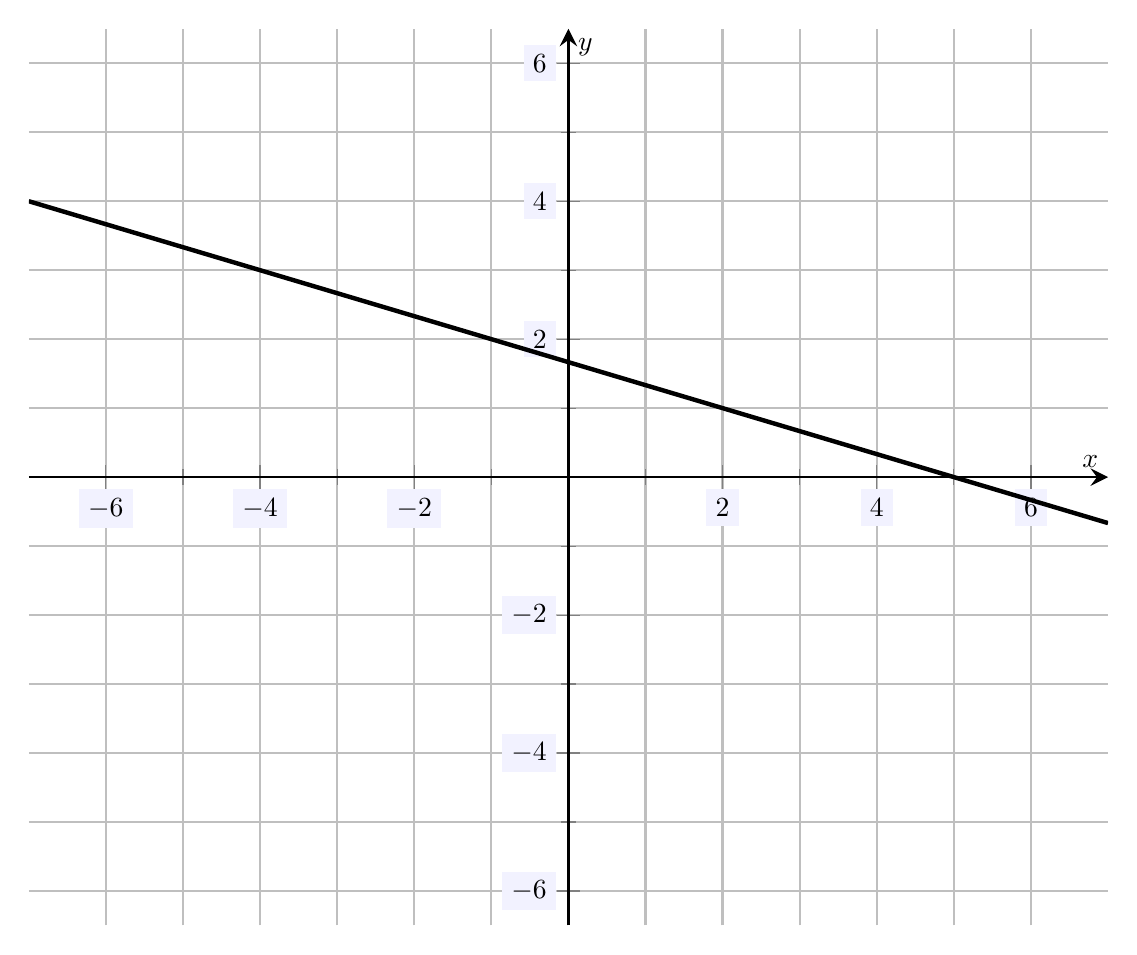
\begin{tikzpicture}[scale=2,every node/.style={scale=0.5}]
	\begin{axis}[
	grid=both,
	axis lines=middle,
	ticklabel style={fill=blue!5!white},
	xmin= -7, xmax=7,
	ymin= -6.5, ymax=6.5,
	xtick={-6,-4,-2,0,2,4,6},
	ytick={-6,-4,-2,0,2,4,6},
	minor tick = {-5,-3,...,5},
	xlabel=\(x\),ylabel=\(y\),
	]
	\addplot[thick, domain= -7:7] {-1/3*x + 5/3};
	\end{axis}
	\end{tikzpicture}
	}
	\]





\newpage





% Problem 7
\problem{10} Solve the following equation for $y$:
	\[
	5x - 3y= 12
	\]






%\printpoints
\end{document}